\chapter{Introduction}
The graph visualization user interface (gvis) of DNA - Dynamic Network Analyzer offers an intuitive and easy to use graph visualization tool with elaborate customization options. Figure \ref{ex:attack} illustrates a sophisticated visualization of a graph modeling network activity. The following chapters will describe how to use gvis and how one may adapt it to specific cases.

\begin{figure} [h]
\centering
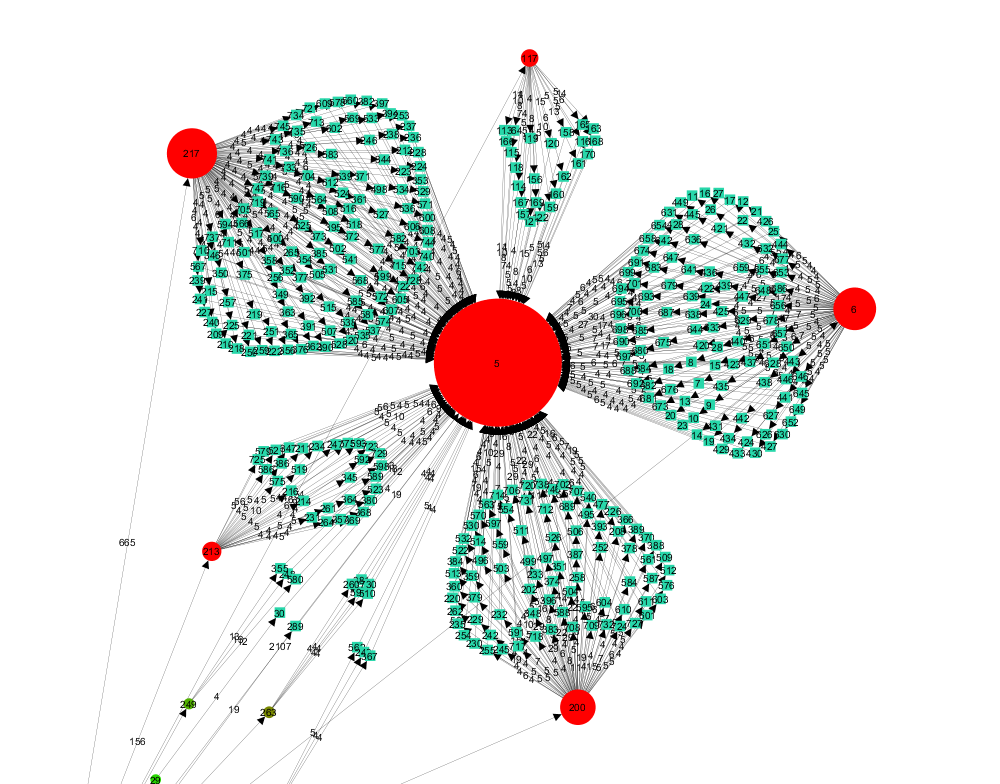
\includegraphics [scale=0.6] {images/attack-example}
\caption{Example of a DDoS-attack modeled as a graph.}
\label{ex:attack}
\end{figure}